% Copyright (c) 2014,2016 Casper Ti. Vector
% Public domain.

\chapter{域名鉴权方案设计}

为了解决现有Web PKI系统中信任不平等构建问题,削弱给予中心化授权机构(CA)过高的信任和权利,提高域名实体对自身证书的管控权,本章将提出基于区块链的域名鉴权方案;首先给出方案的相关概述,对其中的角色和流程进行描述;然后对设计的域名鉴权方案进行详细描述,并对设计的方案进行安全性分析。



\section{方案概述}

\begin{figure}[!htbp]
 	\centering
 	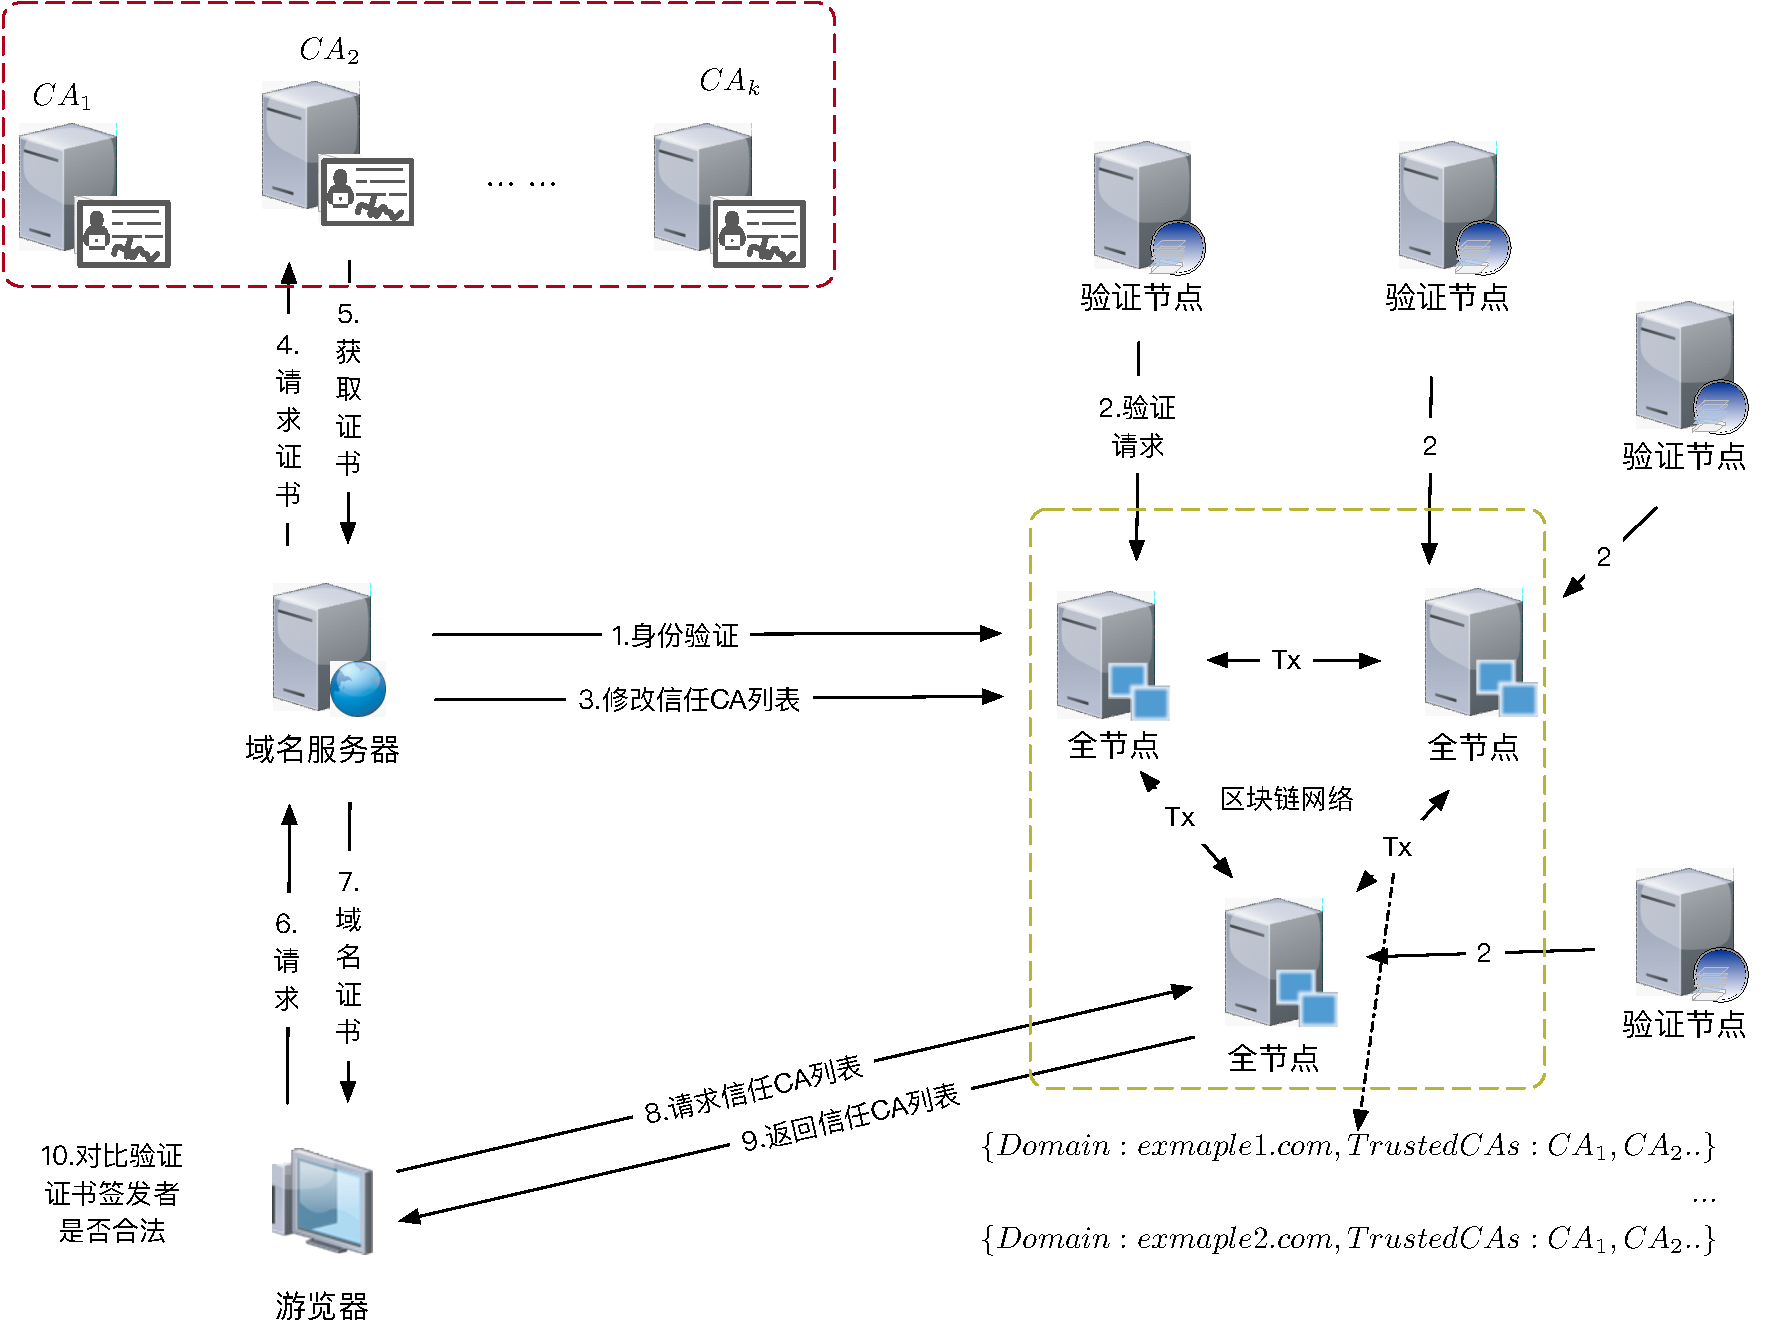
\includegraphics[width = 1\textwidth]{img/arti}
 	\caption{域名鉴权方案}\label{fig:arti}
\end{figure}

在对身份鉴权方案进行详细描述之前,首先对本系统从上层进行透视,了解系统的工作原理和方式,明白设计方案的目的。在本方案中包含的主要实体包括一下几类:
\begin{itemize}
	\item \textbf{授权机构(CA)}:作为证书的管理者,负责对发起证书申请的实体进行证书颁发。
	\item \textbf{证书申请者(域名服务器)}:证书的持有者,依照本文设计的方案进行身份绑定,并将自己信任的CA列表发布在区块链上。
	\item \textbf{证书验证者(游览器)}:与域名完成TLS建立。
	\item \textbf{验证节点}:依据设计的方案完成对域名身份的绑定。
\end{itemize}


域名作为证书的申请者和持有者,在原有的PKI系统中需要向授权机构进行证书的申请操作,以及向与通信的实体提供持有的证书已证明身份。在本方案中,域名将作为核心角色来完成对证书签发相关的控制,方案的整体概况如图\ref{fig:arti}所示。

在域名进行证书申请前,需要通过区块链完成信任列表的存储:首先其向区块链网络发起身份绑定请求,待交易被区块链网络接收后,验证节点对这些请求进行验证;当域名的身份绑定完成之后,域名发送自己信任的CA列表到区块链网络中,完成对可以为自己签发证书CA的控制。

其后域名作为PKI系统中的证书申请者,与在之前的系统中一样向授权机构发起证书申请,授权机构对域名进行身份核实和一系列检查之后完成证书的签发。在该过程中,CA作为证书的签发方,也可以通过区块链来进行证书申请者的信任CA列表查询,来确认自己是否被该申请者纳入到了信任列表之中。但是这样做将对原有PKI系统的CA进行一定的更改,并且这样做并不会对后面的检查造成实质性的影响,只是确保了自身签发证书的合理性,不会影响到证书相关的验证。所以在本方案中并不要求授权机构在完成证书签发的时候通过区块链来做进一步的检查。

当依赖方通过浏览器向域名发起安全连接时,将会获得域名持有的证书;首先和在原有PKI系统中一样,对证书进行签名相关的验证,确认证书是否由可信的授权机构签发。其后,浏览器会向区块链请求该域名的信任CA列表,并将得到的信息与证书进行对比,查看是否由可信的CA签发。


\section{域名鉴权方案设计}

在本方案中,域名需要将自己信任的CA列表记录到区块链上,但是区块链具有去中心化和匿名的特性,域名直接将自己的信任CA放置到区块链上是不具有可信性度,也就是说在区块链上任何人都可以对任何域名进行声明。因此,之前需要完成区块链地址(或者公钥)和域名本身的绑定,实现地址与域名之间的实体认证,完成对域名的鉴权。本文将提供基于验证时间和基于验证次数的鉴权方案。

身份绑定过程大致分为3个步骤:

\begin{enumerate}
	\item 域名发送认证请求到区块链上;
	\item 待交易确认后,根据交易和区块在服务端放置验证;
	\item 验证节点对其进行验证,达到验证期限或者次数后,完成身份绑定。
\end{enumerate}

\subsection{基于验证时间的鉴权方案}

基于验证时间的方案旨在让绑定者提供验证信息持续一段时间,以供所有节点对其进行验证,当提供的验证达到指定时间后,即认为其对该域名服务器的所有权,完成指定地址和域名的绑定。


\noindent\textbf{假设}

假设绑定者A拥有公钥$Pk_A$、私钥$Sk_A$以及域名$example.com$,其需要完成$(Pk_A, example.com)$的绑定;某一验证者B拥有公钥$Pk_B$和私钥$Sk_B$。

\noindent\textbf{交易类型}

在本方案中,包含以下两种类型的交易:

\begin{enumerate}
	\item 绑定请求交易$Tx_{req}$:交易请求者发布绑定请求,包含了自己的公钥$Pk_A$和域名$examle.com$。
	\item 检举交易$Tx_{rep}$:在绑定完成之前,验证节点发现绑定者的验证信息放置不准确,可以提出检举交易,驳回身份绑定。
	\item 验证交易$Tx_{vfy}$:在检举交易发起后,验证者对检举交易进行的验证。
\end{enumerate}

\noindent\textbf{流程}

\begin{figure}[!htbp]
 	\centering
 	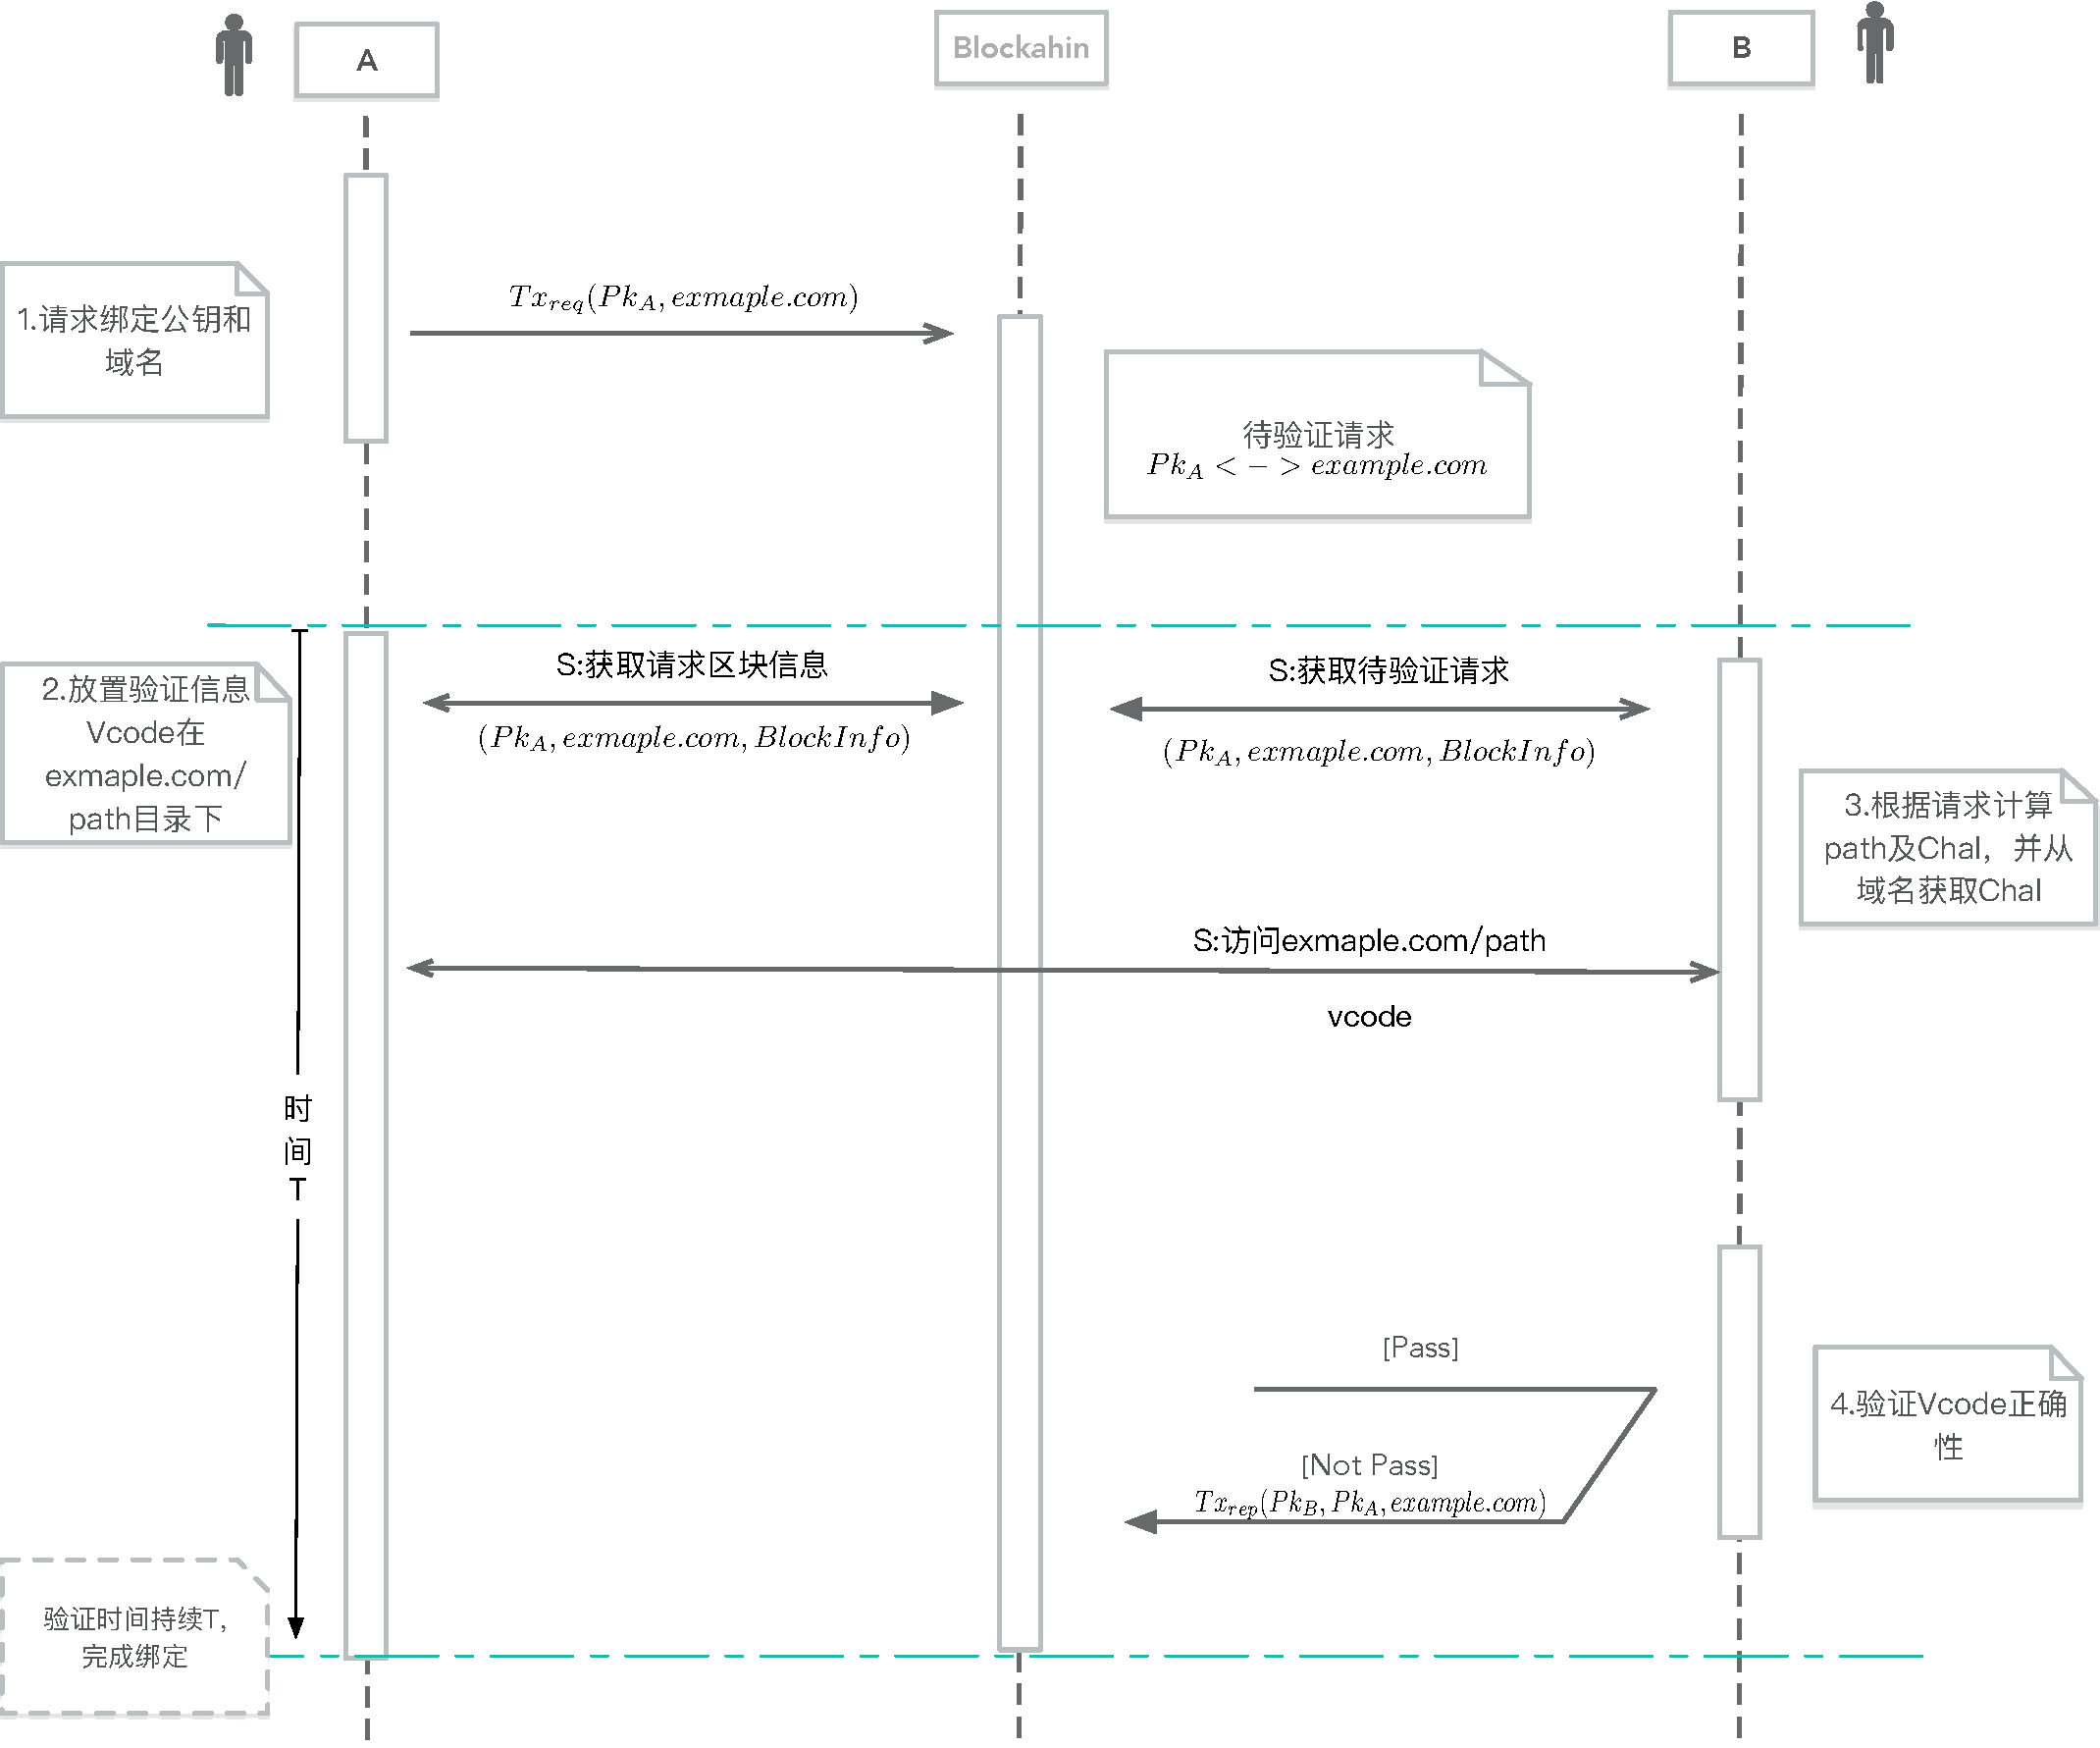
\includegraphics[width = 1\textwidth]{img/time_based_workflow}
 	\caption{基于时间的方案流程图}\label{fig:time_based_workflow}
\end{figure}

绑定的具体流程如图\ref{fig:time_based_workflow}所示,包含以下几步:

\begin{enumerate}
	\item $A$发布绑定交易$Tx_{req}(Pk_A, example.com)$到区块链上;
	\item 根据需要绑定的信息$(Pk_A, example.com)$,计算$(Path, Chal) = F(Pk_A, example.com)$放置在自己控制的域名下,即访问$example.com/Path$即可获取到$Vcode = Sign_{Sk_A}(Chal)$值;
	\item 验证者$B$访问域名验证A是否正确操作,如果不,发送检举交易$Tx_{rep}(Pk_B, Pk_A, example.com)$到区块链;
	\item $A$保持验证时长$T$后,可停止该验证服务,完成绑定。
\end{enumerate}


在该绑定过程中,首先需要绑定者将绑定信息自己的$Pk_A$和自己的域名$example.com$发布到区块链上,将绑定身份信息展现给所有的验证节点,并根据函数$F$生成相关验证内容。我们选择哈希函数$sha256$作为函数原型,将$Pk_A$和$example.com$直接拼接后作为输入,将计算得到的256位哈希值前128位赋值给$Path$、后128位赋值给$Chal$,并且使用自己的私钥对$Chal$进行签名:

\begin{equation}\label{eqF}
Path_{128}||Chal_{128} = sha256(Pk_A||example.com)
\end{equation}

\begin{equation}\label{eqSign}
Vcode = Sign_{Sk_A}(Chal)
\end{equation}

绑定者将以上得到的$Vcode$值放置在网站的$example.com/Path$目录下,作为身份验证的内容,供所有验证节点验证。如果验证节点在验证过程中发现其并没有正确的放置验证信息,将可以通过发送检举信息$Tx_{rep}$对身份绑定消息进行驳回。检举的相关机制会在后面进行详细叙述。


\subsection{基于验证次数的鉴权方案}\label{ver_num}

基于验证次数的方案需要在绑定者发布绑定信息后,选择出合适的验证者,对绑定者的验证信息进行确认,当验证的次数达到规定次数后即可完成身份绑定。

\noindent\textbf{假设}

假设绑定者A拥有公钥$Pk_A$,私钥$Sk_A$以及域名$example.com$,其需要完成$(Pk_A, example.com)$的绑定;某一验证者B拥有公钥$Pk_B$和私钥$Sk_B$。

\noindent\textbf{交易类型}

在本方案由于需要特定验证者完成验证信息的确认,相比于基于时间的验证方案,增加了验证交易类型,包含一下三类交易类型:

\begin{enumerate}
	\item 绑定请求交易$Tx_{req}$:交易请求者发布绑定请求,包含了自己的公钥$Pk_A$和域名$examle.com$。
	\item 检举交易$Tx_{rep}$:在绑定完成之前,验证节点发现绑定者的验证信息放置不准确,可以提出检举交易,驳回身份绑定。
	\item 验证交易$Tx_{vfy}$:验证者在完成验证信息的对比后,在验证通过的情况下发送验证通过的交易。
\end{enumerate}

\noindent\textbf{流程}

基于验证次数的鉴权方案相比于基于验证时间的方案需要验证者更多的和区块链进行交互,在验证过程中需要将验证是否通过的信息提交到区块链上去,绑定流程如图\ref{fig:count_based_workflow}所示,详细流程如下:

\begin{figure}[htbp]
 	\centering
 	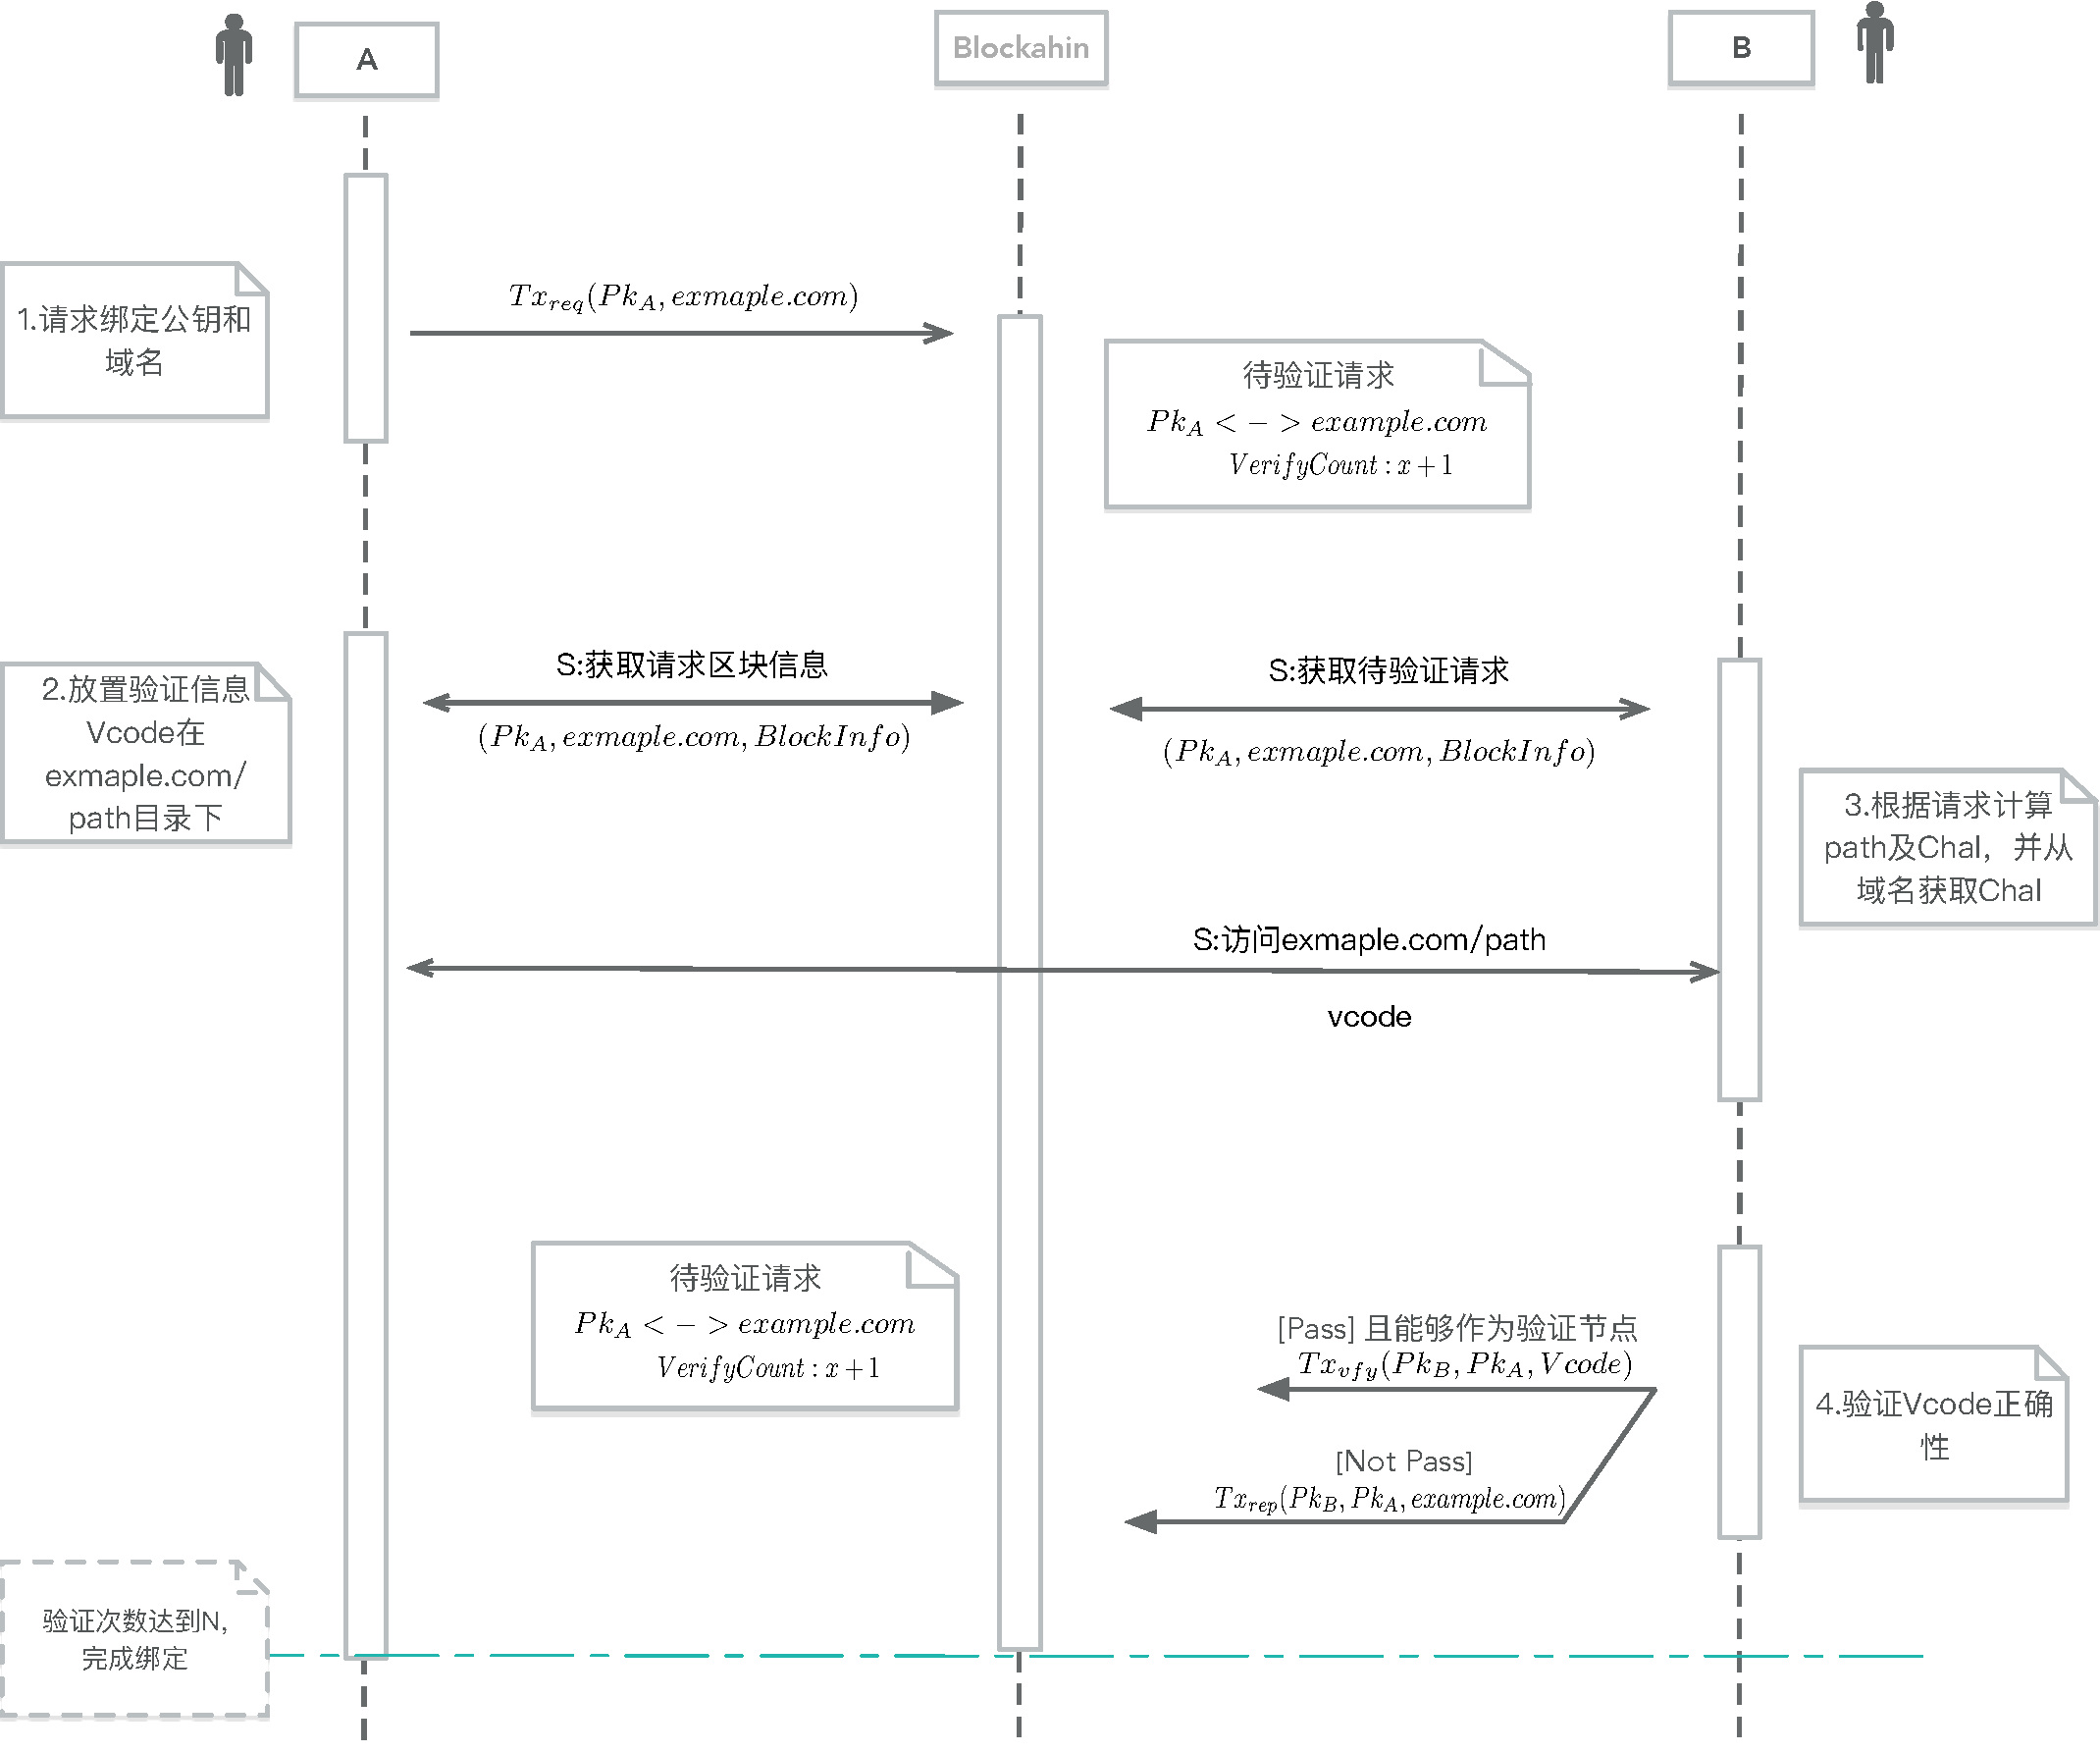
\includegraphics[width = 1\textwidth]{img/count_based_workflow}
 	\caption{基于验证次数的方案流程图}\label{fig:count_based_workflow}
\end{figure}

\begin{enumerate}
	\item $A$发布绑定交易$Tx_{req}(Pk_A, example.com)$到区块链上;
	\item  A获取$Tx_{req}$所在位置区块信息$Info_{block}$,并根据其计算值$(Path, Chal) = F(Info_{rcvBlock})$放置在自己控制的域名下,及访问$example.com/Path$即可获取到$Vcode = Sign_{Sk_A}(Chal)$值;
	\item 根据交易$Tx_{req}$计算符合该条请求的验证者:${v_1, v_2, ... , v_k}$,假设$B$为其中一个验证者
	\item B从$example.com/Path$获取验证内容,提交交易$Tx_{vfy}(Pk_B, Pk_A, Vcode)$ 完成验证。
	\item 在经过$K$个验证过后,即完成绑定。
\end{enumerate}

整体流程和基于时间的方案类似,需要绑定者将自己的公钥$Pk_A$和自己的域名$example.com$发布到区块链上,然后通过公式\eqref{eqF}和\eqref{eqSign}计算得到$Path$和$Vcode$的值放置到自己的服务器上;验证者通过\eqref{eqF}计算获得$Path$、$Chal$和$Pk_A$对验证信息进行确认,确认通过后发送验证交易$Tx_{vry}$到区块链上完成一次验证,待达到验证次数$K$后,即完成身份绑定。


\subsection{检举的工作机制}

在一个p2p的网络中或者一个区块链的网络中,每个用户使用都是一个公钥(即地址),和自身的身份是没有任何关系的,这就是为什么需要设计公钥与域名绑定方案的原因。但是在这样的网络中,任何人都可以发起对任意域名的绑定,为了排除一些错误的绑定或者假冒的绑定,在以上给出两种不同的身份绑定方案中,都是用到了检举交易来完成对这类情况的处理。


当一个诚实的验证节点$C$发现一个虚假的绑定时,他就可以向区块链发起检举交易,和验证交易提交的内容基本一致,只是将最后一项$Vcode$替换为需要检举绑定的域名地址,所以检举交易包含的内容为自身的公钥$Pk_C$和绑定者公钥$Pk_A$和域名$examle.com$。


但是对于一个恶意的验证节点,可能也会对一个真实有效的绑定发起检举交易。为了确认一条检举交易的有效性,需要区块链上验证节点对该条交易给出判断。此时,提交的检举交易和域名提交的绑定交易一样,都是由P2P网络中单一实体提出的待验证的请求,需要网络中的其它实体来进行核实。当检举交易被提交到网络中并被区块所确认,将如同绑定请求一样,随机的选着n个验证者对该请求进行验证,决定本次检举的有效性。


\subsection{验证者的选取}

基于时间的方案中,需要一种选取验证者的规则,避免节点为了自己的利益而不纳入或者滞后其它节点的验证交易;更为重要的是,如果验证节点不是经过一定规则筛选得出的,而是每个节点都可以对绑定身份进行验证的话,在本方案中恶意的绑定者可以使用不同的公钥作为验证节点,然后对恶意绑定进行确认,即发起女巫攻击;同时,正常的验证者为了获得更多的奖励,也会申请尽量多的账户对交易进行验证。

为了避免以上的情况出现,本方案中设计了依据绑定信息随机选择验证节点的方法,保证验证可以有效的进行。当绑定信息被发布到区块链上后,根据绑定信息$Pk_A$、$example.com$和该交易所在位置的区块信息$Info_{rcvBlock}$,将其转换为基准值$hash_{cmp}$:

\begin{equation}\label{eqGenCmpPk}
hash_{cmp} = sha_{512}(Pk_A||example.com||Info_{rcvBlock})
\end{equation}

得到基准值之后,验证节点将通过对纳入该区块之后的区块信息进行签名,来判断自己是否具有成为验证本次请求的权力,判断的方法如\ref{cmpCondition}式所示:


\begin{equation}\label{cmpCondition}
dist_{ham}(Sha_{512}(Sig_{Pr_C}(Info_{curBlock})), hash_{cmp}) <= d + \Delta_t / t_{adjust}
\end{equation}

其中$dist_{ham}(a,b)$表示两个数a和b之间的海明距离;$Pr_C$表示验证节点的私钥;$d$表示初始时的海明距离要求;$\Delta_t$表示从开始收到验证请求已经过去的时间;$t_{adjust}$调整海明距离的时间;$Info_{curBlock}$表示最新块的相关信息;$Sig$为一个unique signature算法。

以上判断方法使得一个验证者可以在每产生一个区块就可以进行一次尝试,判断自己是否能够成为验证节点,同时,随着时间的推移,成为验证节点的难度也在不断减小,保证一定会有验证者被选出。






\subsection{验证交易的附带信息}

验证交易在本方案中起着重要的作用,是验证节点参与到本系统中的重要途径之一。验证节点随时监控区块链上提交的身份绑定请求以及相对应的检举信息,当这两种消息公布到区块链上时,意味着需要验证节点参与到事件的确认当中,每个验证节点都会有机会成为验证该事件的节点。

对于身份绑定请求和检举信息的确认,同时都要提交自身的公钥$Pk_C$和绑定者的公钥$Pk_A$,不同的是一个需要提供验证内容$Vcode$,另外一个需要提供域名$example.com$。在此基础上,还需要验证者提供一个基于容量证明的内容,保证身份不是随意产生的,而是付出一定代价维护的。假设需要提供的容量证明内容为$prf$,其需要满足以下条件:

\begin{equation}\label{pocVerify}
Verify(Pk_C, prf) = Sha_{512}(Pk_A||Vcode/example.com||Info_{curBlock})
\end{equation}

其中$Verify$是容量证明的验证函数。



\subsection{激励机制}

为了促使本方案有足够多的验证节点加入,保证身份绑定能够完整有效的进行,需要对验证节点给予一定的奖励。在验证过程中,如果发现存在未合理放置验证信息的域名,将可以发起检举交易到区块链上,待交易确认后,其可以得到相应的奖励;为保证本系统中的奖励平衡,发起绑定者需要付出一定的代价,而验证者发现错误时,将可以获取得到相应的奖励。

由于这些实体都存在与区块链的网络当中,所有的身份都是公钥(或者公钥转换得到的地址)来表示的;根据前面方案描述的场景,假设域名拥有$Pk_A$,验证者拥有$Pk_B$,以及检举者拥有$Pk_C$,在区块链上上各自都拥有相应的账户余额。

在这些实体在与区块链网络交互的过程中,涉及到对区块链记录进行修改的操作将都会有伴随着余额的变化,相关操作的惩罚和奖励机制如下表\ref{table:reward}所示:

\begin{table}[h] %开始一个表格environment,表格的位置是h,here。   
\centering
\begin{tabular}{|p{1cm}|p{1.5cm}|p{1cm}|p{2.5cm}|p{1cm}|p{2.5cm}|p{3.5cm}|} %设置了每一列的宽度,强制转换。  
 
\hline  
  交易名称 & 发起对象 & 公钥 & 交易含义 & 交易费用 & 后续奖励 & 请求确认后余额\\ %用&来分隔单元格的内容 \\表示进入下一行  
\hline %画一个横线,下面的就都是一样了,这里一共有4行内容  
 $Tx_{req}$ & 域名 & $Pk_A$ & 完成身份绑定 & $-P_1$ & 0 & $Blance(Pk_A) - P_1$ \\
 \hline
 $Tx_{rep}$ & 检举者 & $Pk_C$ & 对身份绑定进行检举& $-P_2$ & $R_1 = \frac{P_1}{2}$ & $Blance(Pk_C) + \frac{P_1}{2}$ \\
 \hline
 $Tx_{vfy1}$ & 验证者 & $Pk_B$ & 对身份绑定进行验证& $-P_3$ & $R_2 = P_3 + \frac{P_1}{K}$ &  $Blance(Pk_B) + \frac{P_1}{K}$ \\
 \hline
 $Tx_{vfy2}$ & 验证者 & $Pk_B$ & 对检举进行确认& $-P_3$ & $R_3 = P_3 + \frac{P_1}{2n}$ &  $Blance(Pk_B) + \frac{P_1}{2n}$ \\
 
\hline  
\end{tabular}  
\caption{激励机制}\label{table:reward} %显示表格的标题 
\end{table} 


第一条规则的设计让身份绑定者需要余额,而不是无限制的随意的在本方案中发起身份绑定操作,从而避免了恶意的破坏者无限度的去发起无效的身份绑定,从而影响本系统中正常身份绑定者的顺利进行;第二条规则是为了防止网络中的验证节点随意的发起检举交易来扰乱正常绑定的完成;第三条规则是对付出验证操作的节点给予奖励,作为吸引更多节点加入的激励机制,但是其在验证之前需要付出一定的余额,防止一些节点对验证过程进行作弊操作;第四条规则和第三条规则类似,属于激励规则,促使更多的节点加入到本系统中。


结合交易代价和后续奖励,可以知道该系统中的所有奖励来源主要来源于身份绑定者域名,而且整个系统在工作的过程中不会凭空产生价值,总的收支是平衡的。



\section{分析与讨论}


%from A Distributed Public Key Infrastructure for the Web Backed by a Blockchain
%or from Accountable Key Infrastructure (AKI)/ A Proposal for a Public-Key Validation Infrastructure.pdf
% or form BKI: Towards Accountable and Decentralized Public-Key Infrastructure with Blockchain
\subsection{安全分析}

\subsubsection{安全模型}

我们假设区块链网络中存在$M$个全节点,其中有$p$占比的全节点被恶意攻击者控制,另外$1-p$的节点为诚实的全节点;验证节点的数量为$N$,其中有$q$占比验证节点被恶意攻击者所控制,另外$1-q$占比数量的验证节点为诚实的节点。%PKI系统中存在$L$个CA,其中某个CA被攻破的概率为$o$。

\subsubsection{51\%攻击}

显然,当$p > 1/2$时,无论底层区块链使用的是PoS还是PoW共识机制,攻击者都可以完成对区块链网络的控制。换而言之,其可以完成对区块中纳入交易的控制,对任意域名发起身份绑定之后,将检举交易不纳入到区块当中,进而通过自己手中持有的验证节点对该绑定进行验证,最终完成对虚假身份的绑定。

\subsubsection{恶意绑定分析}


当一个验证请求被发起后,需要从网络中选取的验证节点进行验证。根据前面验证者的选取过程可以知道,每次进行验证者选取的过程其实一个随机的过程,这里假设我们设计的随机算法是完全随机的,那么选择出$K$节点全部都为恶意节点的概率为:

\begin{equation}\label{Pr_1}
Pr_1 = \prod_{i=0}^{K-1}\frac{qN-i}{N-i}
\end{equation}

也就是说,将会有$1-Pr_1$的概率会产生检举交易。根据方案设计,当检举交易产生时,会根据检举交易的内容进行验证者的选取,将会对本次检举进行半数确认,确认通过的概率为:

\begin{equation}\label{Pr_2}
Pr_2 = \prod_{i=0}^{n/2}\frac{qN-i}{N-i}
\end{equation}

所以当攻击者拥有全网$q$占比的验证节点时,完成一次恶意绑定的概率如式\ref{Pr_all}所示。

\begin{align}
\label{Pr_all}  Pr_{attack} &= Pr_1 + (1-Pr_1) * Pr_2 \\
							&= Pr_1 + Pr_2 - Pr_1 * Pr_2 \\
             				&= \prod_{i=0}^{K-1}\frac{qN-i}{N-i} + \prod_{i=0}^{n/2}\frac{qN-i}{N-i} - \prod_{i=0}^{K-1}\frac{qN-i}{N-i} * \prod_{i=0}^{n/2}\frac{qN-i}{N-i} 
\end{align}


\subsubsection{拒绝绑定分析}

当一个验证请求被发起后,域名正确的放置了验证信息,等待验证者完成验证即可完成对身份绑定。但是,恶意的攻击者可能会对任何验证请求提交检举请求,扰乱绑定的正常进行。在发起恶意的检举之后,能够成功的扰乱本次请求的概率如式\ref{Pr_d}所示。

\begin{equation}\label{Pr_d}
Pr_{denial} = \prod_{i=0}^{n/2}\frac{qN-i}{N-i}
\end{equation}

\subsubsection{攻破域名}

当一个恶意的攻击者将域名攻破时,其可以完成对域名的完全控制,那么在本方案中,就可以完成对信任CA的完全控制。为了ji降低本状况带来的影响,本文建议域名在不同的服务器上放置信任列表变动监测程序,当信任列表发生变化时及时的给出提醒,供域名拥有者进行确认。





\subsection{其它讨论}

\subsubsection{站点对域名服务器的控制权}

为了保证绑定者对域名服务器拥有控制权,在以上方案中,使用提交的$Tx_{req}$来生成验证内容$Path$和$Chal$,保证了验证内容和提交请求的相关性;同时在\eqref{eqF}中使用$sha256$作为随机函数,将提交内容转换为验证内容,该过程是一个不可逆的过程,从验证内容到提交内容的生成是很难完成的,保证了很难通过验证内容去构造提交内容。在放置的验证内容中,$Vcode$是使用绑定公钥对应私钥对$Chal$进行签名得到的,保证了绑定者对私钥的拥有权。


\subsubsection{验证交易的有效性}

基于时间的验证方案中不需要提交者发起验证提交,在发现错误的时候需要发送检举交易;对于基于验证次数的方案而言,需要提交验证内容即$Vcode$,因为有签名的存在,验证节点不能凭空的发送验证交易,需要通过服务器提供的验证信息才能正确的完成验证。

绑定者如果未能正确的放置验证内容,或者通过其它方式公布验证内容,导致验证过程依旧执行,那么其他验证节点可以通过检举交易对其发起检举。


\subsubsection{女巫攻击}

本方案建立在一个P2P的开放式网络中,任何人都可以生成公钥加入到本系统中,成为一个合法验证节点。在第二章中我们知道,一个公开且没有身份管控的开放网络很容易受到女巫攻击;更具体一点,恶意的攻击者可以生成任意多的公私钥对,从而拥有本系统的多个身份,然后在验证过程中增大自己被选为验证节点的可能性;或者恶意攻击者通过在发起绑定前,不断尝试生成公私钥对并挑选出可以成为验证节点的公私钥,然后在发起绑定交易后瞬间完成对绑定请求的确认。

对于上述的第一种情况,在本方案中的任何节点都可以生成任意多的身份,以增大自己的作为验证节点的几率。根据验证者选取公式\ref{eqGenCmpPk}可知,不仅依赖于交易的绑定信息,而且还和交易被确认在区块链上的位置密切相关,所以一个公私钥是否能成为验证者并不能事先决定。对于第二种攻击方式是一样的道理,攻击者无法事先确认成为验证者的要求。

同时,如果有人希望通过拥有多个公私钥对来发起女巫攻击,在发起验证交易还需要提供一个附加信息,其中包含了一个可验证的工作量证明。这意味着如果一个节点想拥有多个身份,就需要投入更多的空间来提供工作量证明所需的内容,很大程度上限制了一个节点所拥能拥有的身份数量。                          

\subsubsection{防定点攻击}

在本方案中,一个公私钥拥有者是否可以成为一个请求的验证者,是通过式\ref{eqGenCmpPk}和式\ref{cmpCondition}来决定。当一个请求发起之后,大家都可以得到共同的基准值$hash_{cmp}$,其无法决定一个公钥拥有者$Pk$与该基准值之间的关系,只有拥有$Pk$对应私钥$Pr$的节点才可以去计算式\ref{cmpCondition},判断自己是否能够为这一次请求进行确认操作。这意味着对于每次请求发出之后,网络中没有人能够去判断谁能为此次请求进行确认;否者,攻击者可以通过对这些确认的验证节点发起比如DDoS攻击或者劫持服务来阻止它们完成验证,进而增大自己成为验证节点的几率。



% \subsubsection{验证时间的选择}

% 在区块链上有确认交易的概念,以保证交易被正确的收录到了区块链中,并在很大程度上达到不可篡改的安全级别\cite{nakamoto2008bitcoin}。假设区块链上的交易确认块数为$\Delta$,出块的平均时间为$T_{avg}$,在一个$\Delta*T_{avg}$的时间之后,交易将被确认有效,在此期间,所有的节点都可以对该条交易的验证内容进行确认,一旦发现不符合的现象,即可发起检举交易,完成检举。

% \subsubsection{验证次数的选择}

% ...





% vim:ts=4:sw=4
